\documentclass{beamer}
\usepackage{tikz}
\usepackage{algorithm,algorithmic}
\renewcommand{\algorithmiccomment}[1]{\bgroup\hfill//~#1\egroup}
\mode<presentation> {

\usetheme{Madrid}


%\setbeamertemplate{footline} % To remove the footer line in all slides uncomment this line
\setbeamertemplate{footline}[page number] % To replace the footer line in all slides with a simple slide count uncomment this line

\setbeamertemplate{navigation symbols}{} % To remove the navigation symbols from the bottom of all slides uncomment this line
}
\usepackage[utf8]{inputenc}
\usepackage{graphicx} % Allows including images
\usepackage{booktabs} % Allows the use of \toprule, \midrule and \bottomrule in tables
\usepackage{subcaption}

%----------------------------------------------------------------------------------------
%	TITLE PAGE
%----------------------------------------------------------------------------------------

\title[k means]{Image compression using $k$-means clustering algorithm} % The short title appears at the bottom of every slide, the full title is only on the title page

\author{Mert ÇIKLA\\CmpE 530} % Your name
\institute[Boun] % Your institution as it will appear on the bottom of every slide, may be shorthand to save space
{
Boğaziçi University \\ % Your institution for the title page
\medskip
}
\date{December 8, 2016} % Date, can be changed to a custom date

\begin{document}

\begin{frame}
\titlepage % Print the title page as the first slide

\end{frame}


\section{Digital Images}
\begin{frame}
\frametitle{Digital Images}
Images are represented by pixels and RGB values.\\

Some cameras use up to 48bits to represent each pixel.\\ 
$3 \times 16$bits for each color $281.5$ trillion colors mean
a typical 20 megapixel image would require without any compression;
$$48\text{bits} \times 2\cdot 10^6 \approx 30 \text{megabytes}$$

We do not need $281.5$ trillion colors in most cases. Most of them are redundant.\\

\end{frame}
\section{Image processing and $k$-means}
\begin{frame}
\frametitle{Image processing and $k$-means}
$k$-means can reduce and choose the colors to represent an image.
\begin{itemize}
\item Turn the colors used in image into a 2$D$ array
\item Use $k$-means on the array to form clusters
\item Each cluster is now a color and we can now use $k$ pixels to represent the image 
\end{itemize}
\end{frame}



\begin{frame}
\frametitle{Image processing examples:1}
$k=20$
\begin{figure}
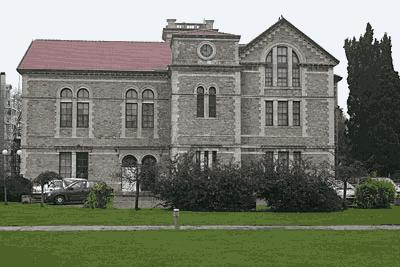
\includegraphics[width=150pt]{boun_compressed.jpg}
\quad 
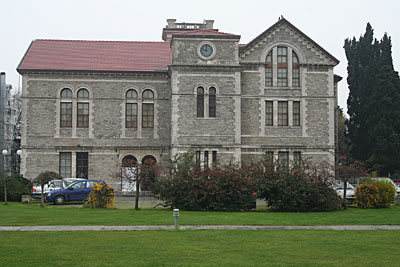
\includegraphics[width=150pt]{boun_4.jpg}
\end{figure}
\end{frame}

\begin{frame}
\frametitle{Image processing examples:2}
Grayscale image with $k=15$ colors
\begin{figure}
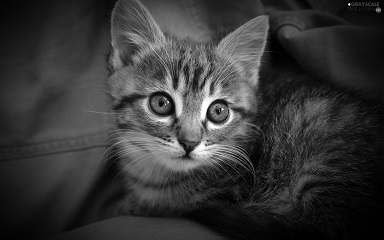
\includegraphics[width=150pt]{kitten.jpg}
\quad 
\includegraphics[width=150pt]{kitten_compressed.jpg}
\end{figure}
\end{frame}

\begin{frame}
\frametitle{Effect of different $k$ and under/over fitting}
\begin{center}
Original Image
\end{center}
\begin{figure}
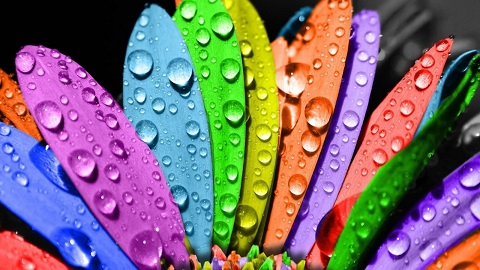
\includegraphics[scale=0.7]{flower.jpg}
\end{figure}
\end{frame}
 

\begin{frame}
\frametitle{Effect of increasing $k$ and under/over fitting}
\begin{center}
Compressed Image with $k$=1
\end{center}
\begin{figure}
\includegraphics[scale=0.7]{flower_compressed_1.jpg}
\end{figure}
\end{frame}

\begin{frame}
\frametitle{Effect of increasing $k$ and under/over fitting}
\begin{center}
Compressed Image with $k$=2
\end{center}
\begin{figure}
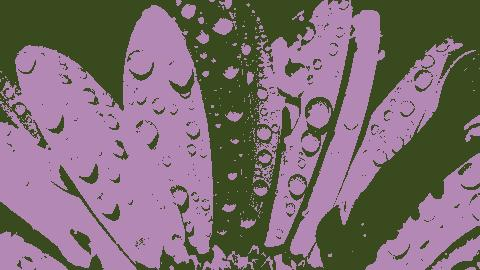
\includegraphics[scale=0.7]{flower_compressed_2.jpg}
\end{figure}
\end{frame}

\begin{frame}
\frametitle{Effect of increasing $k$ and under/over fitting}
\begin{center}
Compressed Image with $k$=3
\end{center}
\begin{figure}

\includegraphics[scale=0.7]{flower_compressed_3.jpg}
\end{figure}
\end{frame}

\begin{frame}
\frametitle{Effect of increasing $k$ and under/over fitting}
\begin{center}
Compressed Image with $k$=4
\end{center}
\begin{figure}
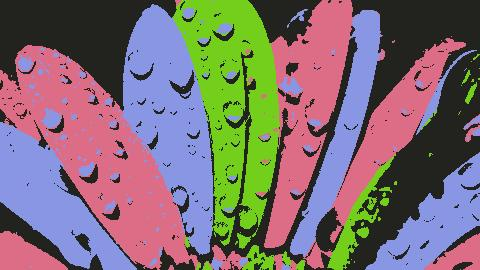
\includegraphics[scale=0.7]{flower_compressed_4.jpg}
\end{figure}
\end{frame}

\begin{frame}
\frametitle{Effect of increasing $k$ and under/over fitting}
\begin{center}
Compressed Image with $k$=5, under fit for most situations
\end{center}
\begin{figure}
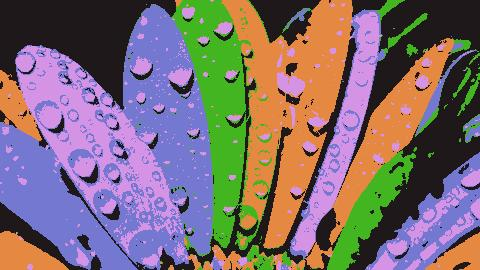
\includegraphics[scale=0.7]{flower_compressed_5.jpg}
\end{figure}
\end{frame}

\begin{frame}
\frametitle{Effect of increasing $k$ and under/over fitting}
\begin{center}
Compressed Image with $k$=7
\end{center}
\begin{figure}
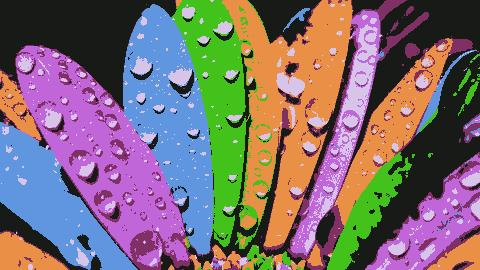
\includegraphics[scale=0.7]{flower_compressed_7.jpg}
\end{figure}
\end{frame}

\begin{frame}
\frametitle{Effect of increasing $k$ and under/over fitting}
\begin{center}
Compressed Image with $k$=10
\end{center}
\begin{figure}

\includegraphics[scale=0.7]{flower_compressed_10.jpg}
\end{figure}
\end{frame}

\begin{frame}
\frametitle{Effect of increasing $k$ and under/over fitting}
\begin{center}
Compressed Image with $k$=20
\end{center}
\begin{figure}

\includegraphics[scale=0.7]{flower_compressed_20.jpg}
\end{figure}
\end{frame}

\begin{frame}
\frametitle{Effect of increasing $k$ and under/over fitting}
\begin{center}
Compressed Image with $k$=50
\end{center}
\begin{figure}
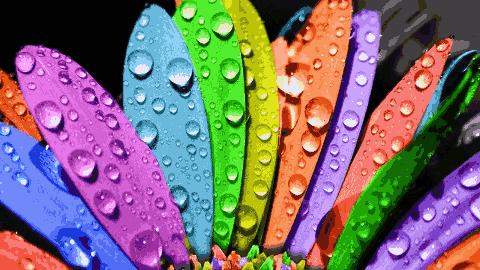
\includegraphics[scale=0.7]{flower_compressed_50.jpg}
\end{figure}
\end{frame}

\begin{frame}
\frametitle{Effect of increasing $k$ and under/over fitting}
\begin{center}
Compressed Image with $k$=100
\end{center}
\begin{figure}
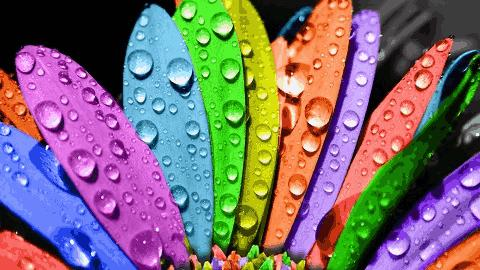
\includegraphics[scale=0.7]{flower_compressed_100.jpg}
\end{figure}
\end{frame}


\begin{frame}
\frametitle{Effect of increasing $k$ and under/over fitting}
\begin{center}
Compressed Image with $k$=200
\end{center}
\begin{figure}
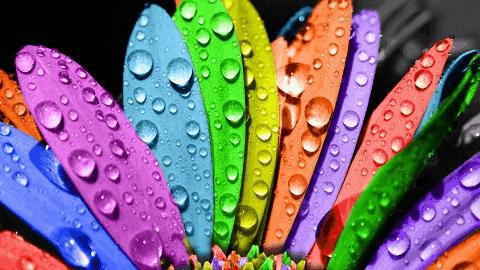
\includegraphics[scale=0.7]{flower_compressed_200.jpg}
\end{figure}
\end{frame}

\begin{frame}
\frametitle{Effect of increasing $k$ and under/over fitting}
\begin{center}
Compressed Image with $k$=200 and the original
\end{center}
\begin{figure}
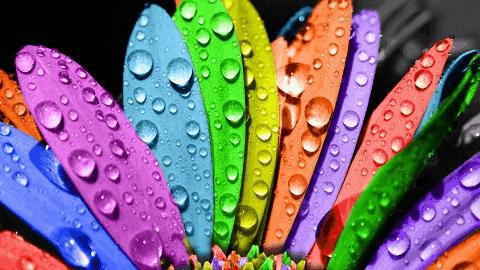
\includegraphics[width=150pt]{flower_compressed_200.jpg}\quad
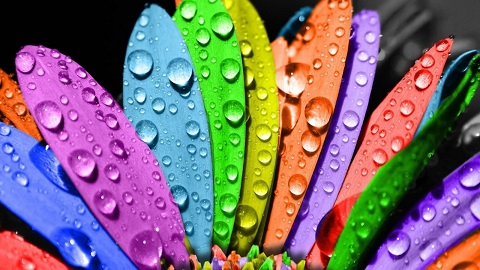
\includegraphics[width=150pt]{flower.jpg}

Even with a $k=200$, data required to represent each pixel reduces to $8$ from $48$\\
Original image is compressed to $\approx \%16$ to its size.

\end{figure}
\end{frame}
\end{document}